\setlength{\footskip}{8mm}

\chapter{Automatic Suspicious Behavior Detection from 
a Small Bootstrap Set}
\label{ch:batch}

\textit{In this chapter, we propose and evaluate a new method for 
automatic identification of suspicious behavior in video surveillance
data. The approach works by constructing scene-specific statistical
models explaining the behaviors occurring in a small bootstrap data
set. It partitions the bootstrap set into clusters then assigns new
observation sequences to clusters based on statistical tests of HMM
log likelihood scores. Cluster-specific likelihood thresholds are
learned rather than set arbitrarily.  In an evaluation on a real-world
testbed video surveillance data set, the method proves extremely
effective, with a false alarm rate of 7.4\% at a 100\% hit rate. The
method is thus a practical and effective solution to the problem of
inducing scene-specific statistical models useful for bringing
suspicious behavior to the attention of human security personnel.}

\section{Introduction}
\label{sec:batch-intro}

Video surveillance is ubiquitous in our lives, but the ongoing
proliferation of surveillance cameras makes it increasingly difficult
to monitor all channels continuously. As the amount of surveillance
video increases, monitoring becomes more expensive and less
effective. Security would be enhanced if it were possible to perform
intelligent filtering of typical events and to automatically bring
suspicious events to the attention of human security personnel.

The goal of automated suspicious event detection, however, requires
some level of human behavior understanding. Many researchers have
attempted to build intelligent systems able to interpret and
understand human
behaviors \shortcite{davis98activity,masoud03recognition,cao04motion,sminchisescu05motion,du06activity,li06behavior,wang06gesture}.
Pre-trained hidden Markov models (HMMs) and other dynamic Bayesian
networks such as conditional random fields (CRFs) have been widely
used in this area, ranging from visual activity
recognition \shortcite{yamato92hmm,sminchisescu05motion,xiang05profiling,vail07activity},
gesture recognition \shortcite{wilson00gesture,gao04dining}, and
unusual activity
detection \shortcite{nair02surveillance,lee03modeling,chan04event,wu05behavior,andrade06crowd,snoek06event,zhang05event,arsic07behavior}. However,
the problem is difficult and remains unsolved, due to the wide range
of activities possible in any given context and the large amount of
variability within any particular activity. In the context of video
surveillance, the problem is even more challenging because behavior
considered normal in one scene might be considered unusual in another
scene.

%Most existing work creates separate models for each distinct a priori
%known class of normal behavior. One example is the work
%of \shortciteA{nair02surveillance}, which performs automated video
%surveillance using HMMs, each modeling a common, pre-defined activity
%in a scene. They classify a sequence as anomalous if the log
%likelihood of the sequence is below a pre-defined threshold for all
%trained HMMs. Other
%work \shortcite{arsic07behavior,lee03modeling,wu05behavior} uses
%support vector machines (SVMs) to model and classify behaviors into
%pre-defined classes.

Here we propose a method for automatic suspicious behavior detection
that utilizes a small bootstrap set in which observation sequences are
manually labeled as normal or suspicious (warranting an operator's
attention).  Using the algorithm from Chapter~\ref{ch:clustering}, we
partition the bootstrap set into clusters of similar sequences and
model each cluster with a simple HMM. We then label each behavior
cluster as normal or possibly suspicious based on the labels of the
individual sequences mapped to the cluster.

After bootstrapping is complete, we assign new observation sequences
to behavior clusters using statistical tests on the log likelihood of
the sequence according to the corresponding HMMs.  A sequence is
considered suspicious if the most likely cluster is already labeled as
suspicious or if its log likelihood according to the most likely
cluster's HMM is too low.  The cluster-specific likelihood threshold
is learned rather than set arbitrarily.

In an evaluation on a real-world video surveillance situation, we find
that, based on a bootstrap set of 150 human motion sequences, our
method is extremely effective at identifying suspicious behavior, with
a false positive rate of 7.4\% at a hit rate of 100\%.  The proposed
method dramatically outperforms traditional machine learning
approaches using the same bootstrap set for training.

Our method is thus a practical and effective solution to the problem
of inducing scene-specific statistical models useful for bringing
suspicious behavior to the attention of human security personnel.

In the rest of this paper, we provide the details of our human
behavior modeling and bootstrapping algorithm in
Section \ref{sec:batch-modeling} and our anomaly detection method in
Section \ref{sec:batch-anomaly-detection}. We demonstrate the feasibility
of the algorithm with an experimental evaluation in
Section \ref{sec:batch-results}, and then discuss and point to future
work in Section \ref{sec:batch-discussion}.

\section{Behavior Model Bootstrapping}
\label{sec:batch-modeling}

Our method for bootstrapping a model of the specific behaviors in a
scene is a batch procedure based on a training video stream acquired
over a short period of time such as one week.  We first perform moving
blob tracking on the training video on the assumption that moving
blobs of sufficient size are people or groups of people.  For each
blob, we extract a sequence of feature vectors describing the blob's
trajectory and appearance over time.  From these data, we
automatically bootstrap a bank of linear HMMs, each model specializing
in one type of behavior.

\begin{figure}[t]
  \centering
  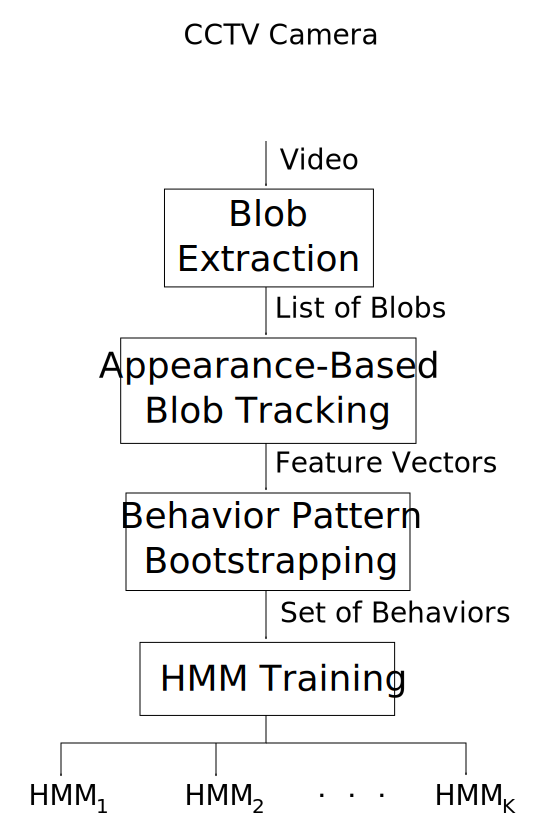
\includegraphics[width=1\linewidth]{figures/behavior-modeling-block-diagram}
  \caption[Block diagram of our overall system.]{\small Block diagram
    of our overall system.}
  \label{fig:behavior-modeling-block-diagram}
\end{figure}

Here we follow the processing steps for motion detection described in
Section \ref{sec:blob-motion-detection} and blob extraction described
in Section \ref{sec:blob-blob-extraction}. 

We define an ``event'' as a contiguous change or motion detected over
some period of time. Extremely short events (occasionally occurring
due to noise) are automatically removed before processing.

Next we use the tracking algorithm previously described in
Section \ref{sec:blob-appearance-based-blob-tracking} to track the
obtained blobs, extract a sequence of feature vectors describing each
blob's trajectory and appearance over time, and automatically
bootstrap a bank of linear HMMs, each model specializing in one type
of behavior.

However, one difference between this chapter and the previous chapter
is that this chapter extends the simple single blob tracking method to
the full multiple blob tracking method described in
Chapter~\ref{ch:blobanalysis}.

\subsection{Behavior Clustering}
\label{sec:batch-behavior-clustering}

After blob tracking, we obtain, from a given video, a set of
observation sequences describing the motion and appearance of every
distinguishable moving object in the scene.  We next partition the
observation sequences into clusters of similar behaviors then model
the sequences within each cluster using a simple linear HMM. 

In this section, we use the method previously described in
Chapter~\ref{ch:clustering}, which first uses dynamic time warping
(DTW) to obtain a distance matrix for the set of observation sequences
then performs agglomerative hierarchical clustering on the distance
matrix to obtain a dendrogram (a binary tree expressing the similarity
structure within the set of observation sequences).  To determine
where to cut off the dendrogram, we traverse the DTW dendrogram in
depth-first order from the root and attempt to model the observation
sequences within the corresponding subtree using a single linear HMM.
If, after training, the HMM is unable to ``explain'' (in the sense
described below) the sequences associated with the current subtree, we
discard the HMM then recursively attempt to model each of the current
node's children. Whenever the HMM is able to explain the observation
sequences associated with the current node's subtree, we retain the
HMM and prune the tree.

A HMM is said to explain or model a cluster $c$ of observation
sequences if there are no more than $N_c$ sequences in $c$ whose
per-observation log-likelihood is less than a threshold $p_c$.  We use
$N_c=10$ in our experiments. The per-observation log likelihood of a
sequence is previously defined in
Section~\ref{sec:clustering-behavior-clustering}.

To determine the optimal rejection threshold $p_c$ for cluster $c$, we
use an approach similar to that of \shortciteA{oates01clustering}. We
generate random sequences from the HMM and then calculate the mean
$\mu_c$ and standard deviation $\sigma_c$ of the per-observation log
likelihood over the set of generated sequences.  For the lengths of
the generated sequences, we simply use the average length of the
sequences in the bootstrap set.  After obtaining the statistics of the
per-observation log likelihood, we let $p_c$ be $\mu_c - z \sigma_c$,
where $z$ is an experimentally tuned parameter that gives us
convenient control over the probability of making Type I errors in
classifying a particular sequence as having been generated by a
particular HMM model.

Our method solves the problem by educing an initial partitioning of
the human behavior observation sequences into groups based on
similarity. Once the set of all behaviors has been partitioned into
groups containing similar sequences, as we shall see, each group can
be modeled individually with a simple statistical model, the linear
HMM. Next, we can use the resulting bank of trained models for anomaly
detection.

The clustering process results in a set of $K$ different typical
behavior clusters ${\cal C} = \{ C_1, C_2, \ldots, C_K \}$ with a set
of $K$ corresponding HMMs ${\cal M} = \{ M_1, M_2, \ldots, M_K \}$.

\section{Anomaly Detection}
\label{sec:batch-anomaly-detection}

In this section we describe our method for anomalous or suspicious
behavior detection. In the \textit{supervised} approach, one would
construct a training set consisting of anomalous and normal behaviors,
build a model, then use the model to classify new behavior sequences
as anomalous or normal.

The pure supervised approach is obviously not suitable, however, when
examples of anomalous behavior are sparse or nonexistent.  In
practical scenarios, the set of possible anomalous behaviors is
infinite in its variety, making it very difficult to acquire a
representative training set.

In the \textit{unsupervised} approach, on the other hand, we would
simply construct a generative model of the normal behavior patterns,
then use the model to classify new behavior sequences as abnormal when
they are ``too far'' in some sense from typical behavior.  For
example, we could use the algorithm described in
Section \ref{sec:batch-behavior-clustering} to construct a bank of
HMMs explaining the normal sequences in a training set of patterns,
then classify new sequences as abnormal or suspicious whenever the
likelihood of the sequence according to the most likely HMM is below
some specific threshold.

The difficulty with the pure unsupervised approach, however, is that
there is no clear way to calibrate the parameters of the ``too far''
criterion.  In practice, one would have to select a conservative
initial distance threshold then fine-tune the threshold to achieve the
best tradeoff between hit and false positive rates.  An inappropriate
initial cutoff could lead to disastrous misses of suspicious behavior
or inundation with false positives.

Since both approaches have limitations, rather than the pure
supervised method or the pure unsupervised method, we instead propose
a \textit{semi-supervised} method that self-calibrates itself from a
small bootstrap set in which each bootstrap sequence is manually
labeled as normal or suspicious by a human operator.  Our method is
simple.  We acquire labels for the bootstrap patterns from the
operator, then we apply the algorithm of
Section \ref{sec:batch-behavior-clustering} to
\textit{both the positive and negative sequences} in the bootstrap
set.  We identify each cluster as a ``normal'' cluster if \textit{all}
of the sequences falling into it are labeled as normal, or identify it
as an ``abnormal'' cluster if \textit{any} of the sequences falling
into it are labeled as abnormal.

For the time complexity of this method, in principle, if we updated
the log likelihood for each model every time we receive a new
observation in constant time, the time complexity would be O($nm$),
where $n$ is the number of observations and $m$ is the number of
models. However, for convenience, we rerun the forward
algorithm \shortcite{rabiner89hmm} on each observation for every
model.

Algorithm \ref{anomaly-detection-algorithm} is a pseudocode summary of
the runtime anomaly detection method. New sequences are classified as
normal if the most likely HMM for the input sequence is associated
with a cluster of normal sequences \textit{and} the $z$-scaled
per-observation log \DIFdelbegin \DIFdel{likelihood of the }\DIFdelend \DIFaddbegin \DIFadd{of the probability of the }\DIFaddend sequence under that most likely
model is greater than a global empirically determined threshold
$\theta_z$.

\begin{algorithm}[t]
  \caption{Anomaly Detection}
  \label{anomaly-detection-algorithm}
  \begin{algorithmic}
    \REQUIRE $\vec{O}$: behavior sequence
    \REQUIRE ${\cal M}$: set of HMMs
    \STATE ${\cal M}_{ab} \gets \{ M \mid M \in {\cal M} \text{~and $M$ is marked abnormal} \}$
    \STATE $( M_{ml}, L_{ml} ) \gets \textsc{Find-Most-Likely-Model}(\vec{O}, {\cal M})$
    \IF{$M_{ml} \in {\cal M}_{ab}$ or $L_{ml} \leq \theta_z$}
      \STATE $\textsc{Alert-Security-Personnel}(\vec{O})$
    \ENDIF
  \end{algorithmic}
\end{algorithm}

\section{Experimental Results}
\label{sec:batch-results}

We created a testbed data set using a CCTV camera with a view of the
front of a building, as seen in
Figure \ref{fig:batch-example-behavior}(a). Videos were recorded at 25
frames per second with a resolution of $320 \times 240$ during working
hours (9:00--17:00) for two weeks. We used the previously-described
techniques to segment the raw video stream into separate videos
containing motion, track blobs, extract features, discretize the
feature vectors, and create observation sequences. We obtained 423
video segments containing 660 observation sequences.

We observed that there are four common activities in this scene:
people walking into the building, people walking out of the building,
people parking bicycles, \DIFdelbegin \DIFdel{and }\DIFdelend people riding bicycles out\DIFaddbegin \DIFadd{, and people walking 
pass by or having interactions with each other}\DIFaddend . 
Figure \ref{fig:batch-example-behavior} shows examples of 
each of these behaviors. In our experiments, we considered all other 
behaviors, such as walking around looking for an unlocked bicycle, to 
be suspicious or abnormal. 

\begin{figure}[t]
  \centering
  \DIFdelbeginFL %DIFDELCMD < \subfloat[]{\includegraphics[width=0.2\textwidth]{figures/example-behavior01.pdf}\label{fig:example-of-scene}}
%DIFDELCMD <   %%%
\DIFdelFL{\hspace{0.05in}
  }%DIFDELCMD < \subfloat[]{\includegraphics[width=0.2\textwidth]{figures/example-behavior02.pdf}}
%DIFDELCMD <   %%%
\DIFdelFL{\hspace{0.05in}
  }%DIFDELCMD < \subfloat[]{\includegraphics[width=0.2\textwidth]{figures/example-behavior03.pdf}}
%DIFDELCMD <   %%%
\DIFdelFL{\hspace{0.05in}
  }%DIFDELCMD < \subfloat[]{\includegraphics[width=0.2\textwidth]{figures/example-behavior04.pdf}}
%DIFDELCMD <   %%%
\DIFdelendFL \DIFaddbeginFL \subfloat[]{\includegraphics[width=0.19\textwidth]{figures/example-behavior01.pdf}\label{fig:example-of-scene}}
  \DIFaddFL{\hspace{0.03in}
  }\subfloat[]{\includegraphics[width=0.19\textwidth]{figures/example-behavior02.pdf}}
  \DIFaddFL{\hspace{0.03in}
  }\subfloat[]{\includegraphics[width=0.19\textwidth]{figures/example-behavior03.pdf}}
  \DIFaddFL{\hspace{0.03in}
  }\subfloat[]{\includegraphics[width=0.19\textwidth]{figures/example-behavior04.pdf}}
  \DIFaddFL{\hspace{0.03in}
  }\subfloat[]{\includegraphics[width=0.19\textwidth]{figures/example-behavior05.pdf}}
  \DIFaddendFL \caption[Examples of common human activities in our testbed
    scene.]{\small Examples of common human activities in our testbed scene.
    (a) Walking in. (b) Walking out. (c) Cycling in. (d) Cycling out. 
    \DIFaddbeginFL \DIFaddFL{(e) Other group activities.}\DIFaddendFL }
  \label{fig:batch-example-behavior}
\end{figure}

To evaluate the effectiveness of our method, we divide the experiments
into two parts: model configuration selection (finding an optimal set
of HMMs to model the bootstrap set) and anomaly detection based on the
HMM bootstrap set. In all of the experiments, we used linear HMMs. We
chose this model structure based on our previous empirical
experience \shortcite{kan08thesis}.

\subsection{Model Configuration Selection}
\label{sec:batch-model-config}

We first manually labeled each of the videos with the categories
``normal'' or ``abnormal.''  For purposes of analyzing the results, we
further subdivided the normal patterns into categories ``walk-in,''
``walk-out,'' ``cycle-in,'' and ``cycle-out,'' but we did not use
these labels for model selection or learning.

Towards model identification, we then performed a series of
experiments with different bootstrap parameter settings and selected
the configuration with the highest accuracy in separating the normal
sequences from the abnormal sequences on the bootstrap sequence set,
as measured by the false positive rate for abnormal sequences.  (Every
bootstrap cluster containing an abnormal sequence is considered
abnormal, so we always obtain 100\% detection on the bootstrap set;
the only discriminating factor is the false positive rate.)  The set
of parameters that we varied were 1) the number of states in each
bootstrap HMM (4--8), 2) the number of sequences used for
bootstrapping (50--200), and the number of tokens used (4--8).

To find the distribution (parameters $\mu_c$ and $\sigma_c$) of the
per-observation log likelihood for a particular HMM, we always
generated 1000 sequences of 150 observations then used a $z$-threshold
of 2.0. We fixed the parameter $N_c$ (the number of deviant patterns
allowed in a cluster) to 10.

A subset of the results of the model configuration selection
experiments are shown in
Figure \ref{fig:batch-some-clustering-results}. Based on the false
positive rate criterion described above, we selected the model
configuration consisting of HMMs with five states and seven tokens
trained on 150 bootstrap sequences.  We arbitrarily chose the model
from one of the 10 trials with this configuration.
Table \ref{tab:batch-bootstrapping-results} shows an example of the
distribution of bootstrap sequences across behavior clusters with the
selected model configuration. In this run, \DIFdelbegin \DIFdel{our method obtained perfect
accuracy }\DIFdelend \DIFaddbegin \DIFadd{we found that, }\DIFaddend with 20 behavior 
clusters\DIFdelbegin \DIFdel{.  }\DIFdelend \DIFaddbegin \DIFadd{, anomalous and typical sequences are always mapped to 
different clusters, although the large number of one-sequence 
clusters means there would be a fairly large amount of manual 
work required to identify them.
}

\DIFaddend We used this model with the
remaining 510 sequences in the anomaly detection experiments described
next.

\begin{figure}[t]
    \centering
    \DIFdelbeginFL %DIFDELCMD < \begin{tabular}{ccc}
%DIFDELCMD < %%%
%DIF <     \includegraphics[scale=0.29]{figures/model-configuration01.png} &
%DIF <     \includegraphics[scale=0.29]{figures/model-configuration02.png} &
%DIF <     \includegraphics[scale=0.29]{figures/model-configuration03.png}\\
%DIF <     \small (a) & \small (b) & \small (c)
    %DIFDELCMD < \includegraphics[scale=0.33]{figures/m5-d7-Nc10-fp-rate} &
%DIFDELCMD <     \includegraphics[scale=0.33]{figures/m5-d7-Nc10-number-of-clusters} %%%
\DIFdelendFL \DIFaddbeginFL \subfloat[]{\includegraphics[scale=0.34]{figures/m5-d7-Nc10-fp-rate}}
    \subfloat[]{\includegraphics[scale=0.34]{figures/m5-d7-Nc10-number-of-clusters.pdf}}\DIFaddendFL \\
    \DIFdelbeginFL %DIFDELCMD < \small %%%
\DIFdelFL{(a) }%DIFDELCMD < & \small %%%
\DIFdelFL{(b) }\DIFdelendFL \DIFaddbeginFL \subfloat[]{\includegraphics[scale=0.34]{figures/m7-d7-Nc10-fp-rate}}
    \subfloat[]{\includegraphics[scale=0.34]{figures/m7-d7-Nc10-number-of-clusters.pdf}}\DIFaddendFL \\
    \DIFdelbeginFL %DIFDELCMD < \includegraphics[scale=0.33]{figures/m7-d7-Nc10-fp-rate} &
%DIFDELCMD <     \includegraphics[scale=0.33]{figures/m7-d7-Nc10-number-of-clusters} %%%
\DIFdelendFL \DIFaddbeginFL \subfloat[]{\includegraphics[scale=0.34]{figures/m9-d7-Nc10-fp-rate}}
    \subfloat[]{\includegraphics[scale=0.34]{figures/m9-d7-Nc10-number-of-clusters.pdf}}\DIFaddendFL \\
\DIFdelbeginFL %DIFDELCMD < \small %%%
\DIFdelFL{(c) }%DIFDELCMD < & \small %%%
\DIFdelFL{(d) }%DIFDELCMD < \\
%DIFDELCMD <     \includegraphics[scale=0.33]{figures/m9-d7-Nc10-fp-rate} &
%DIFDELCMD <     \includegraphics[scale=0.33]{figures/m9-d7-Nc10-number-of-clusters} \\
%DIFDELCMD <     \small %%%
\DIFdelFL{(e) }%DIFDELCMD < & \small %%%
\DIFdelFL{(f) 
  }%DIFDELCMD < \end{tabular}
%DIFDELCMD <   %%%
\DIFdelendFL \DIFaddbeginFL 

    \DIFaddendFL \caption[Subset of model configuration selection results.]{\small
        Subset of model configuration selection results.  Model
        configuration with (a)--(b) five tokens, (c)--(d) seven tokens 
        and (e)--(f) nine tokens. \DIFdelbeginFL \DIFdelFL{Dash }\DIFdelendFL \DIFaddbeginFL \DIFaddFL{Dashed }\DIFaddendFL red, solid green and dash-dot blue 
        lines represent models with five, six and seven states, respectively.  
        Each point is an average over 10 trials.}
    \label{fig:batch-some-clustering-results}
\end{figure}

\begin{table}[t]
  \caption[Example human behavior pattern bootstrapping
    results.]{\small Example human behavior pattern bootstrapping
    results. We used linear HMMs with five states and seven
    tokens. The model consists of 20 clusters. ``W'' means ``walk''
    and ``C'' means ``cycle.''  For the seven clusters containing more
    than one sequence, shown is the distribution of the patterns in
    the cluster over the activities.  The last row shows the
    distribution of the 13 clusters containing only a single sequence
    over the activity categories.}
  \begin{center}
    \begin{tabular}{c|c|c|c|c|c}
      \hline
      Cluster \# & W-in & W-out & C-in & C-out & Other \\
      \hline \hline
      1 & 44 & 0 & 20 & 0 & 0 \\ \hline
      2 & 0 & 37 & 0 & 19 & 0 \\ \hline
      3 & 0 & 0 & 2 & 0 & 0 \\ \hline
      4 & 0 & 0 & 3 & 0 & 0 \\ \hline
      5 & 0 & 0 & 0 & 4 & 0 \\ \hline
      6 & 0 & 0 & 0 & 0 & 6 \\ \hline
      7 & 0 & 0 & 0 & 0 & 2 \\ \hline
      One-seq clusters & 0 & 2 & 6 & 2 & 3 \\ \hline
    \end{tabular}
  \end{center}
  \label{tab:batch-bootstrapping-results}
\end{table}

\subsection{Anomaly Detection}

Here we describe four experiments to evaluate our anomaly detection
method. In Experiment I, we applied our proposed method, as previously
described, to detect anomalous events. In Experiments II, III and IV,
for comparison, we applied traditional machine learning algorithms to
the same problem. We use $k$-nearest neighbors ($k$-NN), Mahalanobis 
classifier, and support vector machines (SVMs).  For
these methods, we use the 150-sequence bootstrap sequence set from
Section \ref{sec:batch-model-config} as training data and test on the
remaining 510 sequences.  Since the main concern in video surveillance
is to detect every unusual event while minimizing the false positive
rate, in every experiment, we calculate an ROC curve and select the
detection threshold yielding the best false positive rate at a 100\%
hit rate. Our experimental hypothesis was that the proposed method for
modeling scene-specific behavior patterns should obtain better false
positive rates than the traditional methods.

\subsubsection{Experiment I: Proposed method}

The red line in Figure \ref{fig:batch-roc-results} represents the ROC
curve for our method as we vary the likelihood threshold at which a
sequence is considered anomalous.  Note that the ROC does not
intersect the point $(0, 0)$ because any sequence that is most likely
under one of the HMMs modeling anomalous sequences in the bootstrap
set is automatically classified as anomalous regardless of the
threshold.

\begin{figure}[t]
  \centering
  \includegraphics[width=0.8\linewidth]{figures/roc-ours-vs-ml-results}
  \caption[Anomaly detection ROC curves. Solid red, dotted green, and dashed 
    blue lines represent ROCs for the proposed method in Experiment I, 
    Mahalanobis classifier for anomaly detection in Experiment III, 
    and SVM-based anomaly
    detection in Experiment IV, respectively.]{\small Anomaly
    detection ROC curves. \DIFdelbeginFL \DIFdelFL{Red}\DIFdelendFL \DIFaddbeginFL \DIFaddFL{Solid red}\DIFaddendFL , \DIFaddbeginFL \DIFaddFL{dotted }\DIFaddendFL green, and \DIFaddbeginFL \DIFaddFL{dashed }\DIFaddendFL blue lines 
    represent ROCs for the proposed method in Experiment I, Mahalanobis 
    classifier for anomaly
    detection in Experiment III, and SVM-based anomaly detection 
    in Experiment IV, respectively.}
  \label{fig:batch-roc-results}
\end{figure}

\begin{table}[t]
  \caption[Anomaly detection results for the proposed method, $k$-NN
    anomaly detection method, Mahalanobis classifier for anomaly detection method, and
    SVM-based anomaly detection method in Experiment I, II, III, and
    IV, respectively.]{\small Anomaly detection results for the
    proposed method, $k$-NN anomaly detection method, Mahalanobis classifier for 
    anomaly detection method, and SVM-based anomaly detection method
    in Experiment I, II, III, and IV, respectively. For the Mahalanobis classifier for 
    anomaly detection method, we include 11 abnormal sequences from
    the bootstrap set in the test set, so the total number of
    positives is 35. TP, FP, TN, and FN are the number of true \DIFdelbeginFL \DIFdelFL{positive}\DIFdelendFL \DIFaddbeginFL \DIFaddFL{positives}\DIFaddendFL , 
    false \DIFdelbeginFL \DIFdelFL{positive}\DIFdelendFL \DIFaddbeginFL \DIFaddFL{positives}\DIFaddendFL , true \DIFdelbeginFL \DIFdelFL{negative}\DIFdelendFL \DIFaddbeginFL \DIFaddFL{negatives}\DIFaddendFL , and false \DIFdelbeginFL \DIFdelFL{negative}\DIFdelendFL \DIFaddbeginFL \DIFaddFL{negatives}\DIFaddendFL , respectively. 
    TPR and FPR stand for true positive rate and false positive rate, 
    respectively.}
  \begin{center}
    \begin{tabular}{c|c|c|c|c|c|c}
      \hline
      Method & TP & FP & TN & FN & TPR & FPR \\
      \hline\hline
      Ours & 24 & 36 & 450 & 0 & 1 & 0.074 \\ \hline
      $1$-NN & 19 & 1 & 485 & 5 & 0.792 & 0.002 \\ \hline
      $2$-NN & 19 & 2 & 484 & 5 & 0.792 & 0.004 \\ \hline
      $3$-NN & 16 & 0 & 486 & 8 & 0.667 & 0 \\ \hline
      $4$-NN & 16 & 1 & 485 & 8 & 0.667 & 0.002 \\ \hline
      $5$-NN & 14 & 0 & 486 & 10 & 0.583 & 0 \\ \hline
      Mahalanobis classifier & 35 & 421 & 65 & 0 & 1 & 0.87 \\ \hline
      SVM & 24 & 228 & 258 & 0 & 1 & 0.469 \\ \hline
    \end{tabular}
  \end{center}
  \label{tab:batch-detection-results}
\end{table}

The ROC reveals that a threshold of $-3.259$ achieves zero false
negatives at a false alarm rate of 0.074.
Table \ref{tab:batch-detection-results} shows the detailed performance
of this model, and Figure \DIFdelbegin \DIFdel{\ref{fig:batch-suspicious-behavior-detected}
}\DIFdelend \DIFaddbegin \DIFadd{\ref{fig:suspicious-behavior-detected}
}\DIFaddend shows an example of a sequence classified as abnormal\DIFdelbegin \DIFdel{(a person
walking around looking for an unlocked bicycle)}\DIFdelend . 

%\begin{table}[t]
%  \caption[Anomaly detection results at 100\% hit rate for the
%    proposed method in Experiment I.]{\small Anomaly detection results
%    at 100\% hit rate for the proposed method in Experiment I.}
%  \begin{center}
%    \begin{tabular}{c|c|c|c|c|c}
%      \hline
%      TP & FP & TN & FN & TPR & FPR \\
%      \hline \hline
%      24 & 36 & 450 & 0 & 1 & 0.074 \\ \hline
%    \end{tabular}
%  \end{center} 
%  \label{tab:batch-detection-results}
%\end{table}

\begin{figure}[t]
  \centering
  \begin{tabular}{ccccc}
    \includegraphics[scale=0.24]{figures/case-1-suspicious-0187} &
    \includegraphics[scale=0.24]{figures/case-1-suspicious-0208} &
    \includegraphics[scale=0.24]{figures/case-1-suspicious-0225} &
    \includegraphics[scale=0.24]{figures/case-1-suspicious-0249} &
    \includegraphics[scale=0.24]{figures/case-1-suspicious-0267} \\
    \small Frame 187 & 
    \small Frame 208 & 
    \small Frame 225 & 
    \small Frame 249 & 
    \small Frame 267 \\
    \includegraphics[scale=0.24]{figures/case-2-suspicious-0188} &
    \includegraphics[scale=0.24]{figures/case-2-suspicious-0334} &
    \includegraphics[scale=0.24]{figures/case-2-suspicious-0344} &
    \includegraphics[scale=0.24]{figures/case-2-suspicious-0353} &
    \includegraphics[scale=0.24]{figures/case-2-suspicious-0377} \\
    \small Frame 188 & 
    \small Frame 334 & 
    \small Frame 344 & 
    \small Frame 353 & 
    \small Frame 377 \\
    \includegraphics[scale=0.24]{figures/case-3-suspicious-0173} &
    \includegraphics[scale=0.24]{figures/case-3-suspicious-0197} &
    \includegraphics[scale=0.24]{figures/case-3-suspicious-0233} &
    \includegraphics[scale=0.24]{figures/case-3-suspicious-0246} &
    \includegraphics[scale=0.24]{figures/case-3-suspicious-0268} \\
    \small Frame 173 & 
    \small Frame 197 & 
    \small Frame 233 & 
    \small Frame 246 & 
    \small Frame 268
  \end{tabular}
  \caption[Example anomaly detected by the proposed method in
    Experiment I.]{\small Example anomaly detected by the proposed
    method in Experiment I.  The \DIFaddbeginFL \DIFaddFL{first row represents the }\DIFaddendFL sequence 
    \DIFdelbeginFL \DIFdelFL{contains }\DIFdelendFL \DIFaddbeginFL \DIFaddFL{containing }\DIFaddendFL a person walking around looking for an unlocked 
    bicycle. \DIFaddbeginFL \DIFaddFL{The second row represents the sequence containing a 
    person walking out of the building then walking back into it. 
    The last row represents a person walking in and looking around 
    then walking out.}\DIFaddendFL }
  \DIFdelbeginFL %DIFDELCMD < \label{fig:batch-suspicious-behavior-detected}
%DIFDELCMD < %%%
\DIFdelendFL \DIFaddbeginFL \label{fig:suspicious-behavior-detected}
\DIFaddendFL \end{figure}
\DIFaddbegin 

\DIFadd{I have performed some brief experimentation to determine how the 
size of bootstrap set affects the results. I found that with more bootstrap 
data we tend to discover more compact behavior classes, leading to better 
anomaly detection rates in practice.
}

\DIFadd{However, since a larger bootstrap set will generally contain more 
variable behavior, our approach consequently creates more models to 
handle the more variable set of patterns. The effect is that we
require more interaction with the operator determine whether each 
behavior cluster is normal or abnormal.
}

\DIFadd{In this sense, the ``optimal'' bootstrap set size would thus be a 
size sufficient to include most typical behaviors (1--2 days) but 
no more.
}\DIFaddend 

\subsubsection{Experiment II: $k$-NN}

In this experiment, we tested the ability of a more traditional
machine learning algorithm, $k$-nearest neighbors, to detect the
anomalies in our testbed data set using the same division of sequences
into training and testing as in Experiment I.  As the distance
measure, we used the same DTW measure we used for hierarchical
clustering of the bootstrap patterns in our method.  We varied $k$
from 1 to 5.  The results are shown in
Table \ref{tab:batch-detection-results}. While the false positive rates are much
lower than those obtained in our method, the hit rates are
unacceptable.  For $k$-NN to be a practical anomaly detection method,
we would have to adjust it.  For example, we could impose a distance
threshold beyond which a pattern is considered anomalous even if a
majority of the nearest neighbors are normal.

%\begin{table}[t]
%  \caption[$k$-NN anomaly detection results in Experiment II.]{\small
%    $k$-NN anomaly detection results in Experiment II.}
%  \begin{center}
%    \begin{tabular}{c|c|c|c|c|c|c}
%      \hline
%      $k$ & TP & FP & TN & FN & TPR & FPR \\
%      \hline \hline
%      1 & 19 & 1 & 485 & 5 & 0.792 & 0.002 \\ \hline
%      2 & 19 & 2 & 484 & 5 & 0.792 & 0.004 \\ \hline
%      3 & 16 & 0 & 486 & 8 & 0.667 & 0 \\ \hline
%      4 & 16 & 1 & 485 & 8 & 0.667 & 0.002 \\ \hline
%      5 & 14 & 0 & 486 & 10 & 0.583 & 0 \\ \hline
%    \end{tabular}
%  \end{center} 
%  \label{tab:kNN-results}
%\end{table}

\subsubsection{Experiment III: Mahalanobis Classifier}

In this experiment, we classified sequences as normal or anomalous
using a Gaussian density estimator derived from principal components
analysis (PCA).  Since PCA requires a fixed-length input vector, we
calculated, for each sequence in the testbed data set, a summary
vector consisting of the means and standard deviations of each
observation vector element over the entire sequence.  With seven
features in the observation vector, we obtained a 14-element vector
summarizing each the sequence.  After feature summarization, we
normalized each component of the summary vector by z-scaling. Then,
since we are performing probability density estimation for the normal
patterns, we applied PCA to the 139 normal sequences in the bootstrap
set.  We chose the number of principal components accounting for 80\%
of the variance in the bootstrap data. Finally, we classified the
remaining 521 test sequences using a Mahalanobis classifier to calculate 
the Mahalanobis distance of each sequence's summary vector to the mean of
the normal bootstrap patterns' summary vectors.

The green line in Figure \ref{fig:batch-roc-results} is the ROC curve
obtained by varying the Mahalanobis distance threshold, and
Table \ref{tab:batch-detection-results} shows detailed results for
anomaly detection at a 100\% hit rate.  The high false positive rate
at this threshold and the overall poor performance in the ROC analysis
show that the Mahalanobis classifier is clearly inferior to our proposed 
method.

%\begin{table}[t]
%  \caption[PCA-based anomaly detection results in Experiment
%    III.]{\small PCA-based anomaly detection results in Experiment
%    III.}
%  \begin{center}
%    \begin{tabular}{c|c|c|c|c|c}
%      \hline
%      TP & FP & TN & FN & TPR & FPR \\
%      \hline\hline
%      35 & 421 & 65 & 0 & 1 & 0.87 \\ \hline
%    \end{tabular}
%  \end{center}
%  \label{tab:pca-detection-results}
%\end{table}

\subsubsection{Experiment IV: SVMs}

Here we used the same summary vector technique used in Experiment III
but performed supervised classification using support vector
machines. We used the radial basis function kernel implementation in
LIBSVM \shortcite{CC01a} with grid search for the optimal
hyperparameters using five-fold cross validation on the training set
(150 sequences). The blue line in Figure \ref{fig:batch-roc-results}
is the ROC curve obtained by varying the threshold on the signed
distance to the separating hyperplane used for classification as
normal or abnormal.  Table \ref{tab:batch-detection-results} shows the
detailed anomaly detection results for SVMs at a 100\% hit rate.
Although the results are clearly better than those obtained from
$k$-NN or PCA, they are also clearly inferior to those obtained in
Experiment I.

%\begin{table}[t]
%  \caption[SVM anomaly detection results in Experiment IV.]{\small SVM
%    anomaly detection results in Experiment IV.}
%  \begin{center}
%    \begin{tabular}{c|c|c|c|c|c}
%      \hline
%      TP & FP & TN & FN & TPR & FPR \\
%      \hline \hline
%      24 & 228 & 258 & 0 & 1 & 0.469 \\ \hline
%    \end{tabular}
%  \end{center}
%  \label{tab:svm-detection-results}
%\end{table}

\section{Discussion}
\label{sec:batch-discussion}

In this chapter, we have proposed and evaluated a new method for
bootstrapping scene-specific anomalous human behavior detection
systems.  The method requires minimal involvement of a human operator;
the only required action is to label the patterns in a small bootstrap
set as normal or anomalous.  On a testbed data set acquired in a
real-world video surveillance situation, with a bootstrap set of 150
sequences, the method achieves a false positive rate of merely 7.4\%
at a hit rate of 100\%.  The experiments demonstrate that with a
collection of simple HMMs, it is possible to learn a complex set of
varied behaviors occurring in a specific scene.

\FloatBarrier

% --- Maybe use later ---

%In more recent years, research has started to focus on the problem of
%unsupervised analysis and clustering of behaviors in a particular
%scene for a variety of purposes including anomaly detection,
%surveillance, and classification. \shortciteA{zhong04detection} treat
%video segments as documents and cluster the documents based on
%co-occurrence information. \shortciteA{li06behavior} cluster human
%gestures by constructing an affinity matrix using dynamic time warping
%(DTW) \shortcite{sakoe78dtw}, then they apply the normalized-cut
%algorithm to cluster the gestures. \shortciteA{hautamaki08clustering}
%apply DTW and use the resulting pairwise DTW distances as input to a
%hierarchical clustering process in which $k$-means is used to
%fine-tune the output.

%\shortciteA{swears08clustering} propose hierarchical
%HMM-based clustering to find and cluster motion trajectories and
%velocities for surveillance video in a highway interchange
%scene. \shortciteA{xiang05profiling} model the distribution of
%activity data in a scene using a Gaussian mixture model (GMM) and
%employ the Bayesian information criterion (BIC) to select the optimal
%number of behavior classes prior to HMM
%training. \shortciteA{kan10clustering} cluster human behaviors using
%DTW and hierarchical clustering and then perform statistical tests to
%find the optimal number of human behavior classes using HMMs.

%In this paper, we propose an effective method for incremental learning
%of normal human behavior as events occur. We find the optimal set of
%human behaviors using DTW and HMMs in a top-down hierarchical
%fashion. Our method improves upon the state of the art in intelligent
%video surveillance applications by bootstrapping human behavior
%classification and anomaly detection modules in a given
%installation. Once a set of initial clusters and corresponding HMMs
%representing typical behavior is created, we perform statistical tests
%on the observation sequence's likelihood according to each HMM
%model. When the likelihood is low according to all of the pre-existing
%clusters, we consider the observation sequence to be anomalous and
%alert a human operator. When the likelihood is sufficiently high for
%one of the pre-existing models, we incrementally update the sufficient
%statistics for that model. We perform support vector machine (SVM)
%classification of the log-likelihood vectors constructed from the set
%of initial HMMs in order to improve detection rates.

%The existing work most similar to ours is the incremental learning
%approach of \cite{xiang08incremental}, who model the activity in a
%scene incrementally after initialization using a small bootstrapping
%dataset; however, both normal and abnormal activities are explicitly
%modeled and classified using a log-likelihood ratio test (LRT). Our
%approach does not require an a priori model of anomalous human
%behavior.  Since anomalous behavior in general scenes is rare and
%diverse, we cannot learn a model for it; we instead detect deviations
%from typical behavior. We consider observation sequences with
%likelihoods below threshold as abnormal. The likelihood thresholds are
%learned rather than set arbitrarily.

% Related works using other methods besides HMMs
% \cite{davis98activity} build an application for human activity
% recognition using the principal component analysis (PCA) to model an
% optical flow field of motions.  \cite{masoud03activity} use the
% work of \cite{ju96motion} to track five human body parts.  Then
% they also apply PCA technique to recognize actions. To classify
% human actions, they compress the training actions, and compute the
% distance between coefficients for a testing action and the
% coefficients of every example action, then choose the minimum
% distance.  \cite{cao04motion} use support vector machines (SVMs) to
% recognize online human motion. Each processed frame of a video is
% classified and labeled separately using SVMs. Then the resulting
% labels are used to determine the motion type of the video through
% majority voting within a sliding window.  \cite{li06behavior}
% propose a method based on space-time image features for automatic
% behavior modeling and recognition. The behavior templates are built
% and used to perform the classification.  \cite{du06activity}
% propose an approach to recognize interaction activities between two
% people based on dynamic Bayesian network (DBN). They add the state
% duration with a reasonable distribution into the model to solve some
% drawbacks from the conventional HMM such as limited performance to
% model long-range process.  Conditional random fields (CRFs) have
% been extended from the natural language processing to a range of
% areas like gesture recognition \cite{wang06gesture} and activity
% recognition \cite{sminchisescu05motion, vail07activity}.
% \cite{sminchisescu05motion} recognize human motion using
% discriminative conditional random field (CRF) and maximum entropy
% Markov models (MEMM).  \cite{vail07activity} apply conditional
% random fields (CRF) for activity recognition in the robot tag
% domain.  \cite{wang06gesture} extend the conditional random fields
% (CRFs) to incorporate with hidden structures for human gesture
% recognition.

% \cite{yamato92hmm} apply discrete HMMs to recognize tennis
% strokes. They train a separate HMM for each action. The correct
% action will yield the highest log-likelihood given the trained
% model.  \cite{wilson00gesture} apply continuous HMMs to recognize
% human gestures in an online fashion. They modify the Baum-Welch
% algorithm to be able to update parameters at runtime.
% \cite{gao04dining} also apply continuous HMMs to recognize dining
% activity in a nursing home.  They define states topology to describe
% stages in dining activities, then identify instances of eating using
% the trained HMM.  \cite{chan06event} present a HMM-based approach
% to detect rare events in aerial video.  Rather than modeling motion
% trajectories directly, they model the spatio-temporal relations
% between objects and uncertainty in observations. Since it is
% difficult to model and differentiate the invariant relationships of
% objects from incidental activities when training data is lacking.
% \cite{snoek06event} propose a method for automatically recognizing
% usual events on stairs and detecting anomalous events such as people
% miss one step or people slip off one step.  They train a single
% continuous HMM on all normal sequences and use a threshold to detect
% anomalies. Additionally, in the experiments, they applied a
% conditional random field (CRF) to compare the detection results.
% \cite{andrade06event} present an automatic method for modeling
% crowd scenes as well as detecting abnormal events. They use the
% combination of the foreground mask and optical flow information to
% only consider the flow vectors inside the foreground objects. After
% that they perform PCA on the optical flow fields of each frame to
% get the activity pattern. They measure the similarity between video
% segments using spectral clustering based on the likelihood given by
% a multi-observation HMM (MOHMM), and then they group the segments
% into $K$ different classes.  They train a MOHHM per class. Then an
% abnormal event is detected if the likelihood given by a bank of
% MOHMM is less than the detection threshold.
% \cite{arsic07behavior}develop a video surveillance application to
% monitor human behaviors in an airplane situation. They use a
% multi-class SVM to model and classify behaviors into the pre-defined
% classes. Because of unknown start and end state or the length of
% motion, their classification is performed by windowing the resulting
% time series of features without any overlap.

% \cite{arsic07behavior} also model and classify behaviors into the
% pre-defined classes using a multi-class support vector machine
% (SVM).

% \cite{xiang05profiling} proposed a HMM-based approach to model
% visual behavior and detect anomalies in a scene without manual
% labeling.

% Works using the extened HMMs \cite{brand97chmm} exploit coupled
% hidden Markov models (CHMMs) to deal with the causal connections
% among multiple temporal processes. In this paper, the author use
% CHMMs to model two-handed actions and to classify gestures into 3
% categories which are single whip, brush knee, and cobra. Their
% experiments presented that CHMMs is superior compared to
% conventional HMMs in terms of training speeds, model likelihoods,
% and robustness to initial conditions. CHMMs use fully-connected
% state space.  \cite{brand00momchmm} propose a multi-observation and
% mixture+counter hidden Markov model (MOMC-HMM).  This kind of HMM is
% used to factorize the observation space. The authors present that
% their framework capable of learning models of office activity and
% outdoor traffic. In this paper, they also demonstrate how this
% framework can be adapted to infer hidden state from extremely
% ambiguous images. For example, it can infer both 3D body pose and
% orientation from image sequences of low resolution silhouettes.
% \cite{xiang05profiling} also employ this kind of HMM in their work
% to learn behavior patterns in a corridor scene, and detect anomalies
% such as a person sneaking into the office area without using an
% entry card.  \cite{vogler01language} propose parallel hidden Markov
% models (PaHMMs). For this kind of HMM, the hidden state space is
% factorized into ``state channels" corresponding to multiple
% independent temporal processes. Consequently, the channels can be
% trained completely independently, and later they can be combined at
% recognition time. Since they apply PaHMMs to recognize American sign
% language (ASL), it is unnecessary to provide examples of all
% possible combinations of phonemes at training time.  Thus, ASL can
% be modeled independently. Their experiments demonstrate that their
% approach outperforms conventional HMMs in dealing with this
% problem. However, the factorizability hypothesis is invalid in most
% cases, particularly when facing the group or interactive activities.
% \cite{gong03activity} propose dynamically multi-linked hidden
% Markov model (DML-HMM). The DML-HMM targets connecting a subset of
% essential hidden state variables across multiple temporal processes
% instead of being fully connected as in the case of a CHMM. The state
% transition matrices are factorized using Schawarz's Bayesian
% information criterion (BIC) \cite{schwarz78bic}. The number of
% unnecessary parameters can be reduced for better network structure
% discovery. Their experiments in this paper presented that DML-HMM
% outperforms a MOMC-HMM, a PaHMM, and a CHMM in modeling group
% activities in a cluttered outdoor scene.

% \cite{zhang05event} propose a method for unusual event detection
% using semi-supervised adapted HMMs. They train an usual event model
% and then used the maximum a posteriori (MAP) to adapt the models as
% well as model unusual event models in a top-down hierarchical
% fashion.  At each iteration, they split the usual event model into
% two models: one represents an usual event model, and the other one
% represents an unusual event model. Then they keep repeating the
% steps until they obtain the desired number of iterations. This
% method does not need explicitly labeled unusual event data.
